%!TEX root = main.tex

\section{Asynchronous advantage actor-critic methods}
\subsection{Methodology}

The asynchronous advantage actor-critic (A3C) algorithm~\cite{mnih2016asynchronous}
 trains multiple agents in parallel and update shared
target policy network and value network. 
Through the asynchronous update, the training can be stabilized 
and accelerated. The actor-critic methods means that each time
the action taken by policy network is "criticized"
by the value network. During the training, each agent conduct a 
roll-out play for a few time steps (say 5). At then end of each 
roll-out play or episode, the advantage and discounted reward were
computed and updates the target policy and value network parameters
through the cumulated gradients in this roll-out play. Several agents
was trained in different copy of same environments and send the updates
to the target networks. For more details, please refer to the paper[Algorithm S3]~\cite{mnih2016asynchronous}.



 % It is a policy-based model-free reinforcement learning method. 
%  This algorithm maintains a policy $\pi
% (a_{t}|s_{t};\theta)$ and the estimate of the value function
% $V(s_{t};\theta_{v})$, where $\theta$ and $\theta_{v}$ are the parameters.
% These two parameters are learned by taking the gradient of $\log \pi
% (a_{t}|s_{t};\theta) A(s_{t},a_{t};\theta,\theta_{v})$ with respect to
% $\theta^{\prime}$. The update of $\pi (a_{t}|s_{t};\theta)$ and
% $V(s_{t};\theta_{v})$ happens either after every $t_{max}$ actions or when a
% terminal state is reached. Combining with the idea in deep learning, we use a
% convolutional neural network that has one softmax output for the policy $\pi
% (a_{t}|s_{t};\theta)$ and one linear output for the value function
% $V(s_{t};\theta_{v})$.	

% The structure of policy network is shown as in Table.\ref{table.cnn_detail}:
% \begin{table}[!ht]
% 	\centering
% 	\caption{CNN detail}
% 	\label{table.cnn_detail}
% 	\begin{tabular}{c|c|c|c}
% 		\textbf{Type} & \textbf{size} & \textbf{\# filters} & \textbf{activation} \\ \hline
% 		convolution & $5\times5$ & 32 & Relu \\ 
% 		max pooling & $2\times2$ &  &  \\
% 		convolution & $5\times5$ & 32 & Relu \\
% 		max pooling & $2\times2$ &  &  \\
% 		convolution & $4\times4$ & 64 & Relu \\
% 		max pooling & $2\times2$ &  &  \\
% 		convolution & $3\times3$ & 64 & Relu \\
% 		fully connected & 512 &  & PRelu \\
% 		softmax &  &  & 
% 	\end{tabular}
% \end{table}




\subsection{experimental results}


Firstly, we modified the implementation of A3C from \href{https://github.com/ppwwyyxx/tensorpack}{tensorpack} repository and
apply this implementation to three environments to verify the effectiveness of this methods.
The experimental results are illustrated at the following links for three environments:
% Fig~\ref{fig:A3C_baselines}. Please also
% see the video animation by clicking the captions under each figures. 
% The results are acquired by a pre-trained model and then follow the A3C models,
\href{https://gym.openai.com/evaluations/eval_i9E40nAQuOTiSa0bxYBA#reproducibility}{Breakout-v0}, 
\href{https://gym.openai.com/evaluations/eval_mvXuxP13SSacO01UIhsg#reproducibility}{Pong-v0} and 
\href{https://gym.openai.com/evaluations/eval_Gva8XrEvTQi63KOd5Gyq1Q#reproducibility}{Phoenix-v0}, respectively.

Secondly, we implement our own A3C from scratch to two OpenAI gym environments, CartPole-v0 and Pong-v0.


\begin{figure}[h!]
\centering
\begin{tabular}{c c}
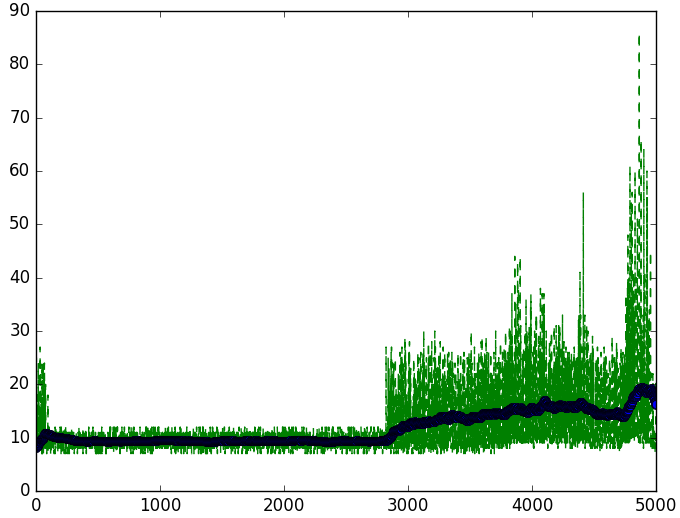
\includegraphics[width=0.22\textwidth]{./fig/myA3C_cartpole_rewardsplot.png} &
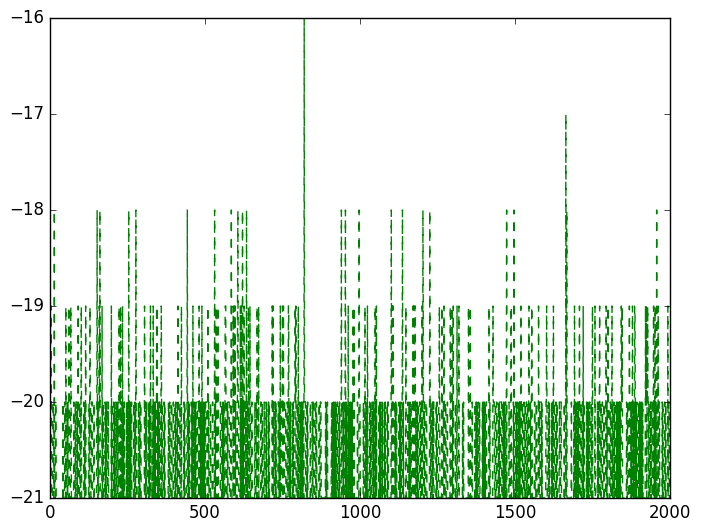
\includegraphics[width=0.22\textwidth]{./fig/myA3C_pong_rewardsplot.png}\\
(a) Cartpole-v0 & (b) Pong-v0  \\
\end{tabular}
\caption{The results of our A3C implementations.}
\label{fig:A3C_baselines}
\end{figure}




% \begin{figure}[h!]
% \centering
% \begin{tabular}{c}
% 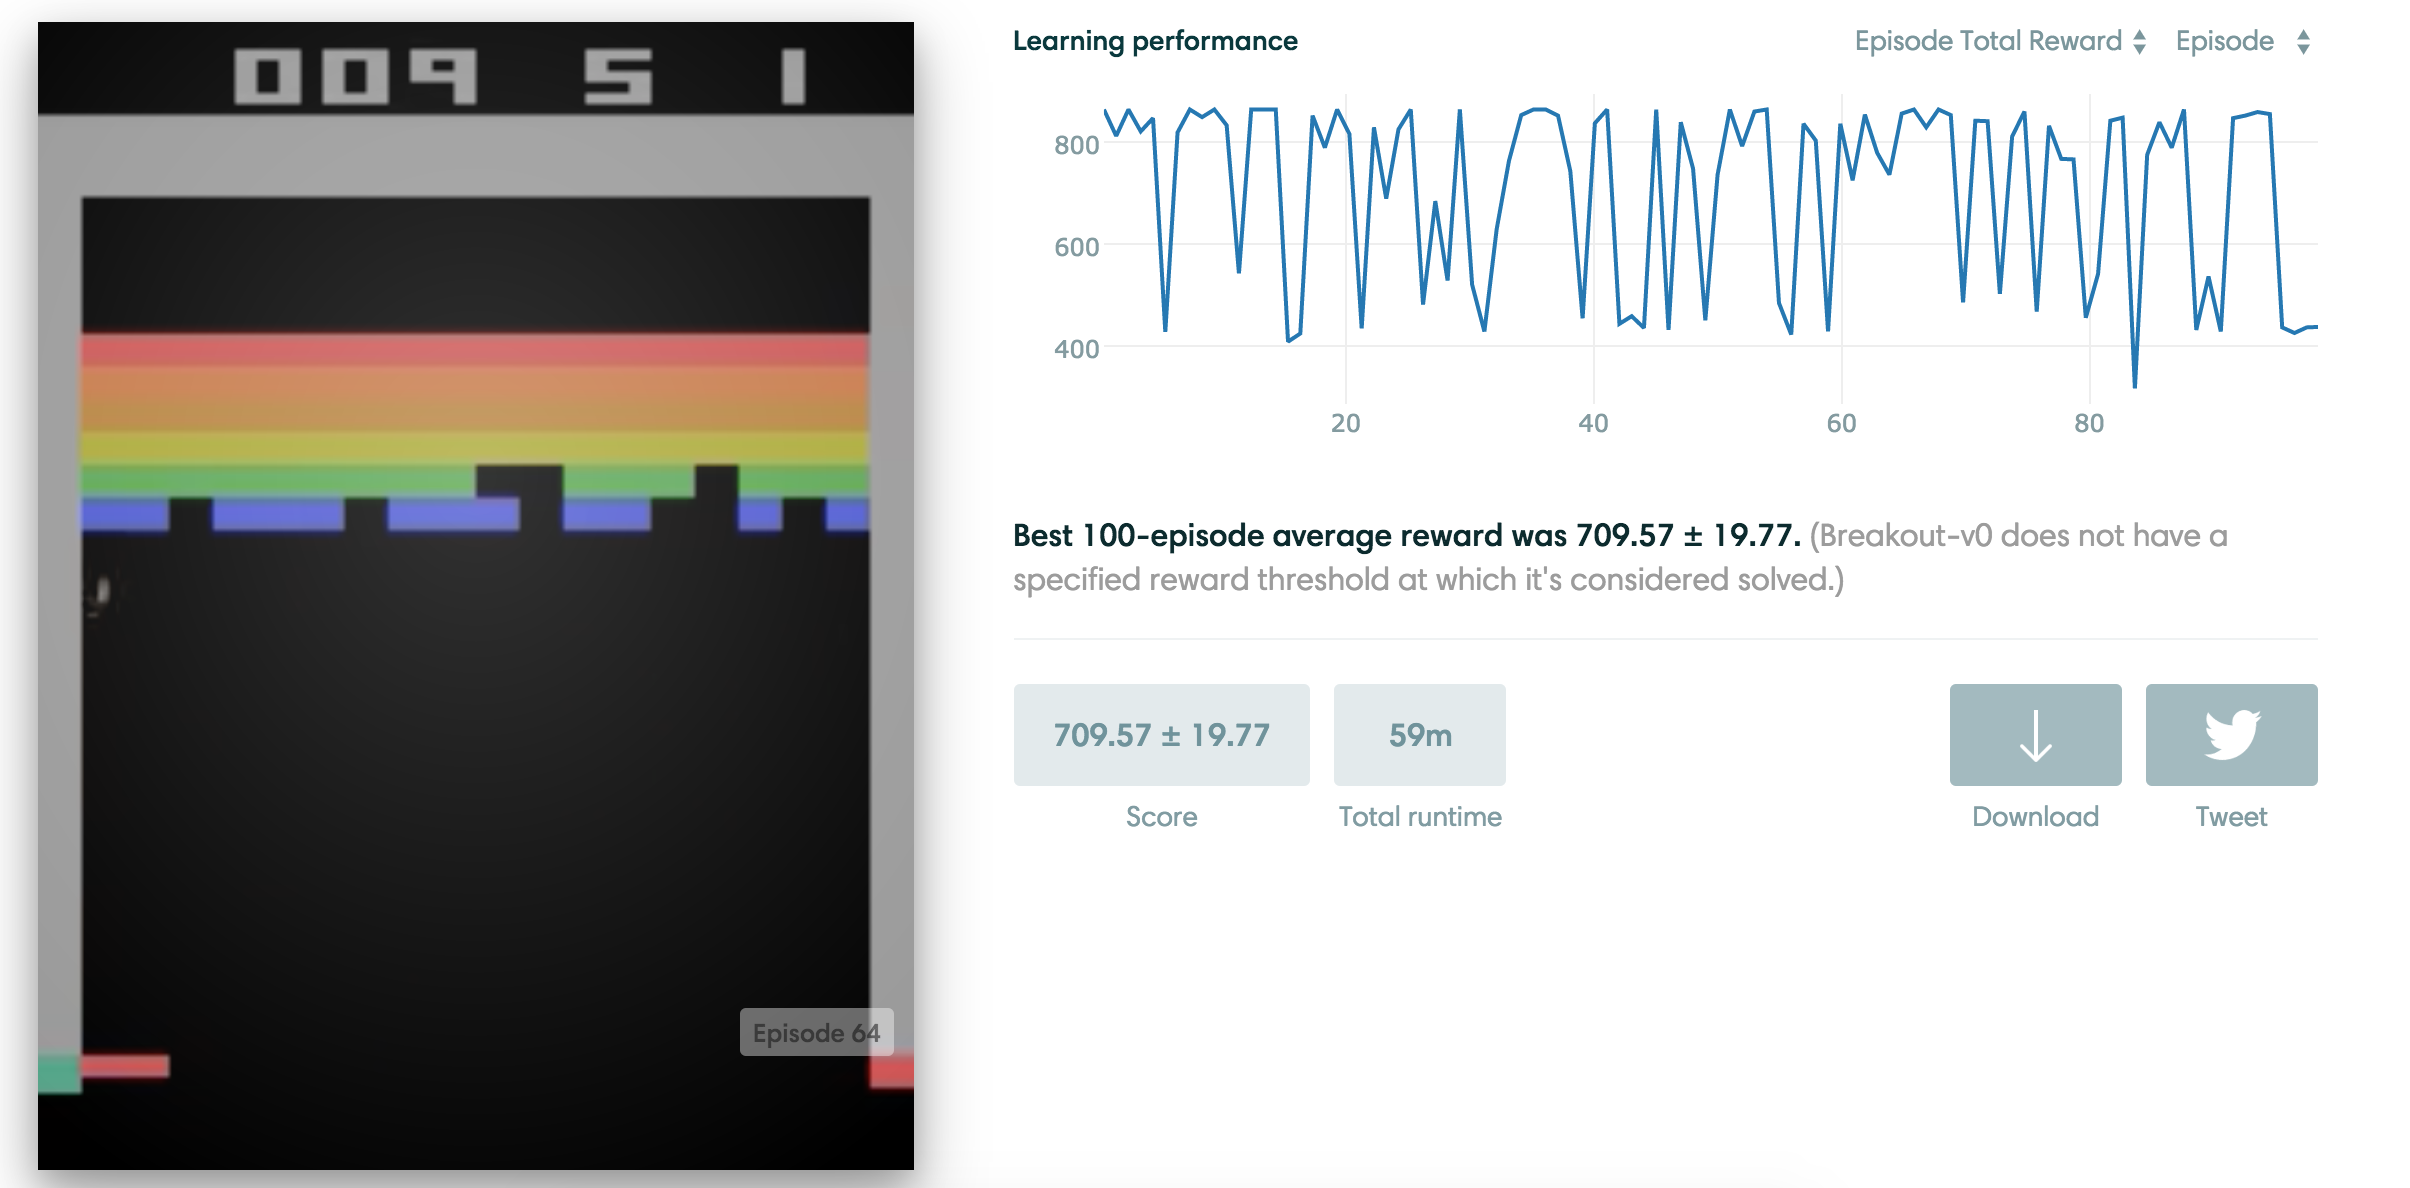
\includegraphics[width=0.49\textwidth]{./fig/A3C_Breakout-v0.png} \\
% (a) \href{https://gym.openai.com/evaluations/eval_i9E40nAQuOTiSa0bxYBA#reproducibility}{Breakout-v0} \\
% 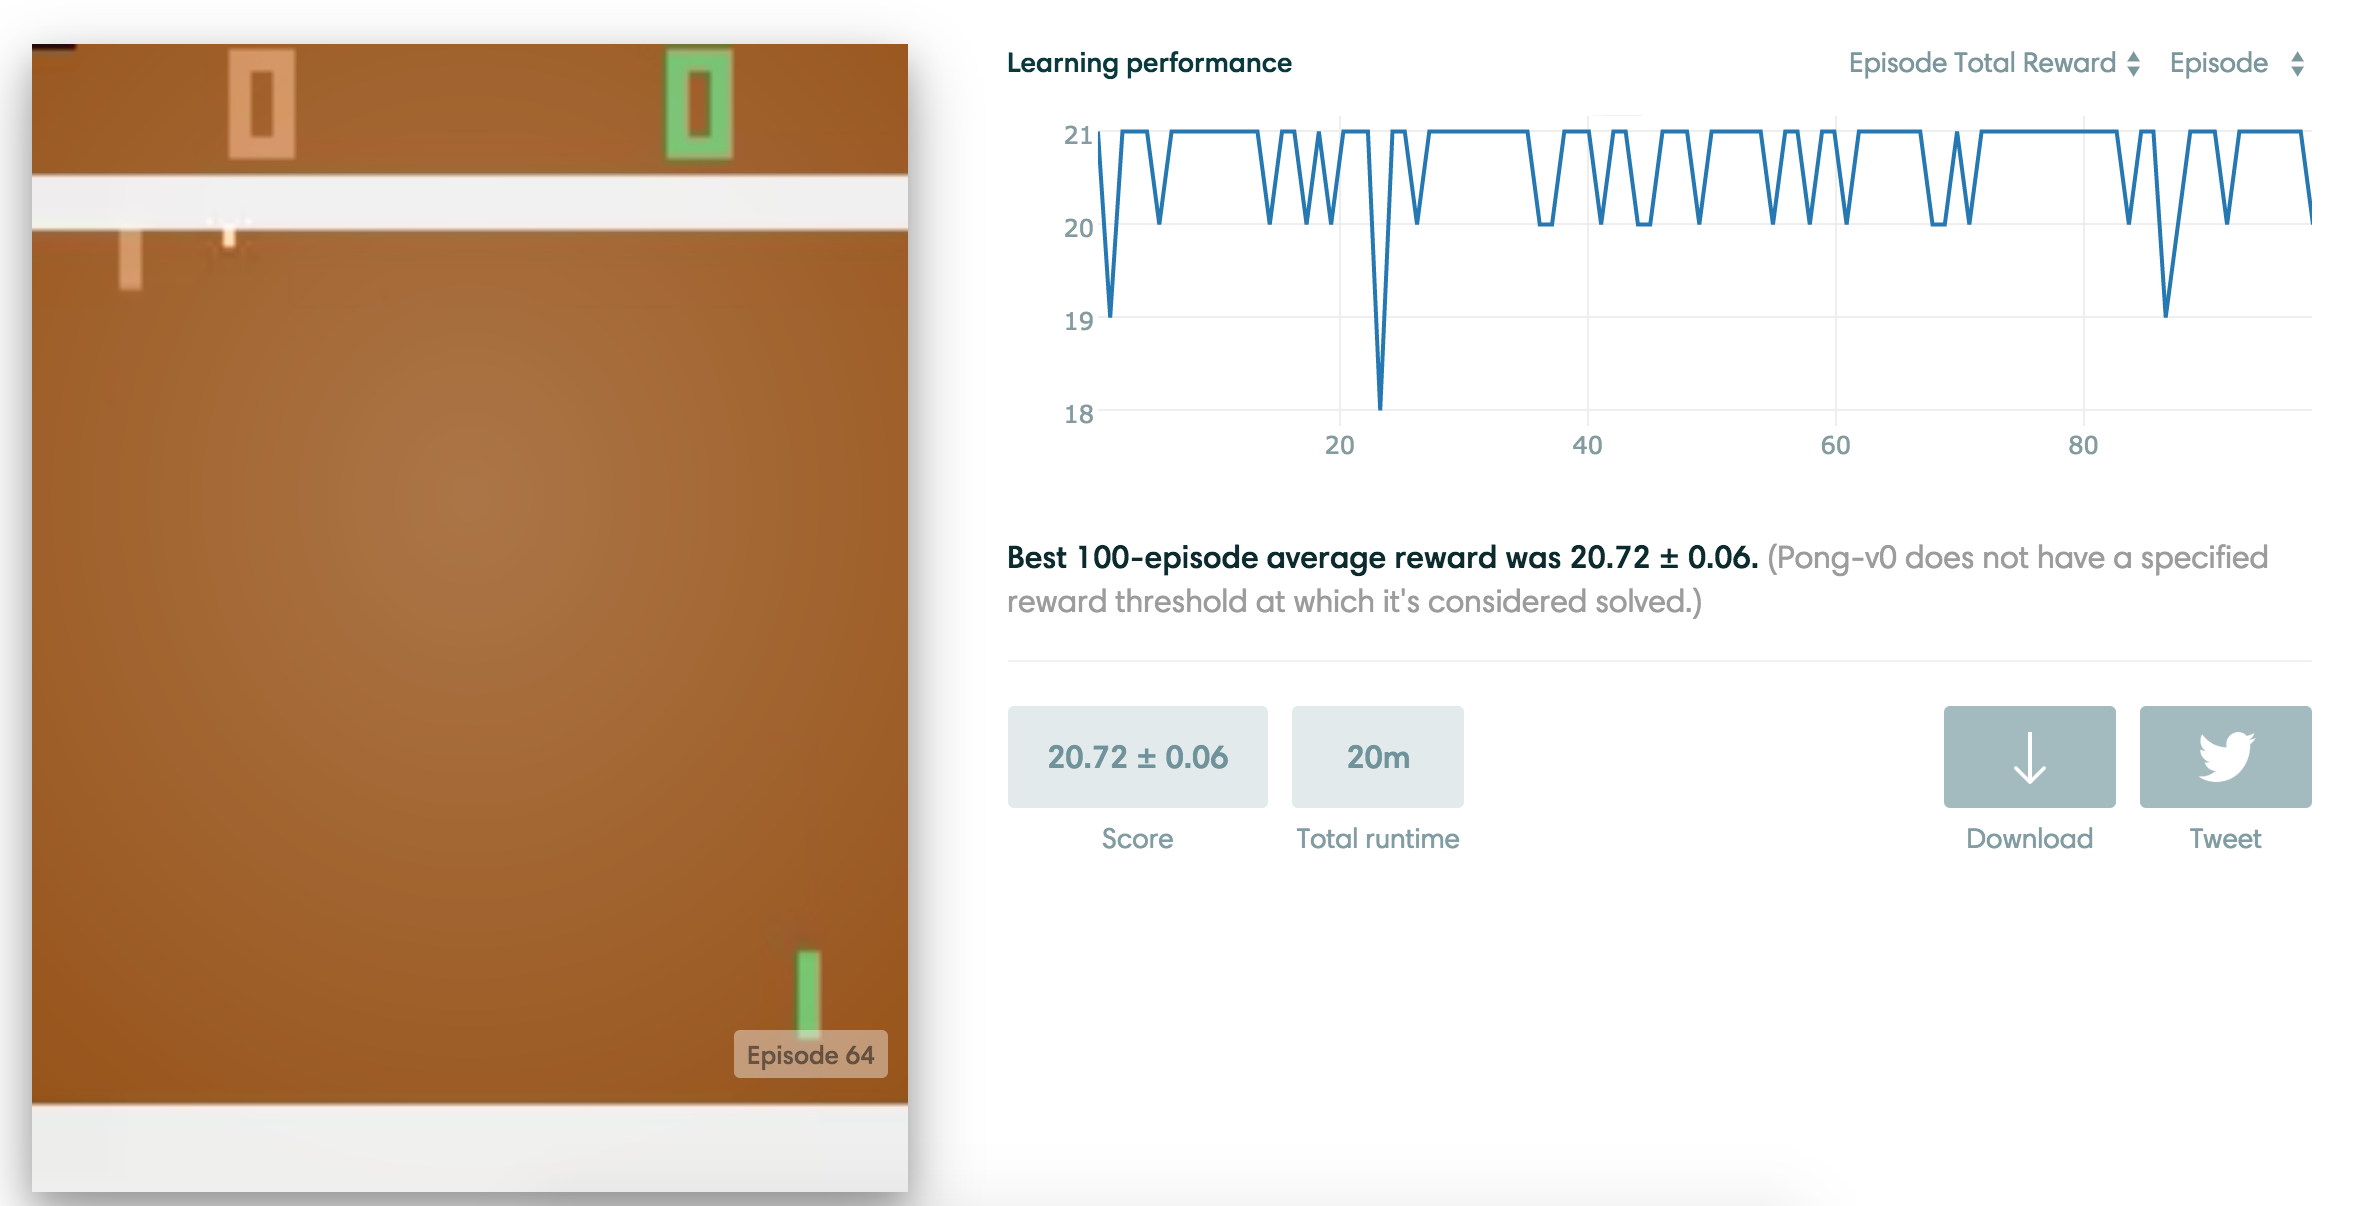
\includegraphics[width=0.49\textwidth]{./fig/A3C_Pong-v0.png} \\
% (b) \href{https://gym.openai.com/evaluations/eval_mvXuxP13SSacO01UIhsg#reproducibility}{Pong-v0} \\
% 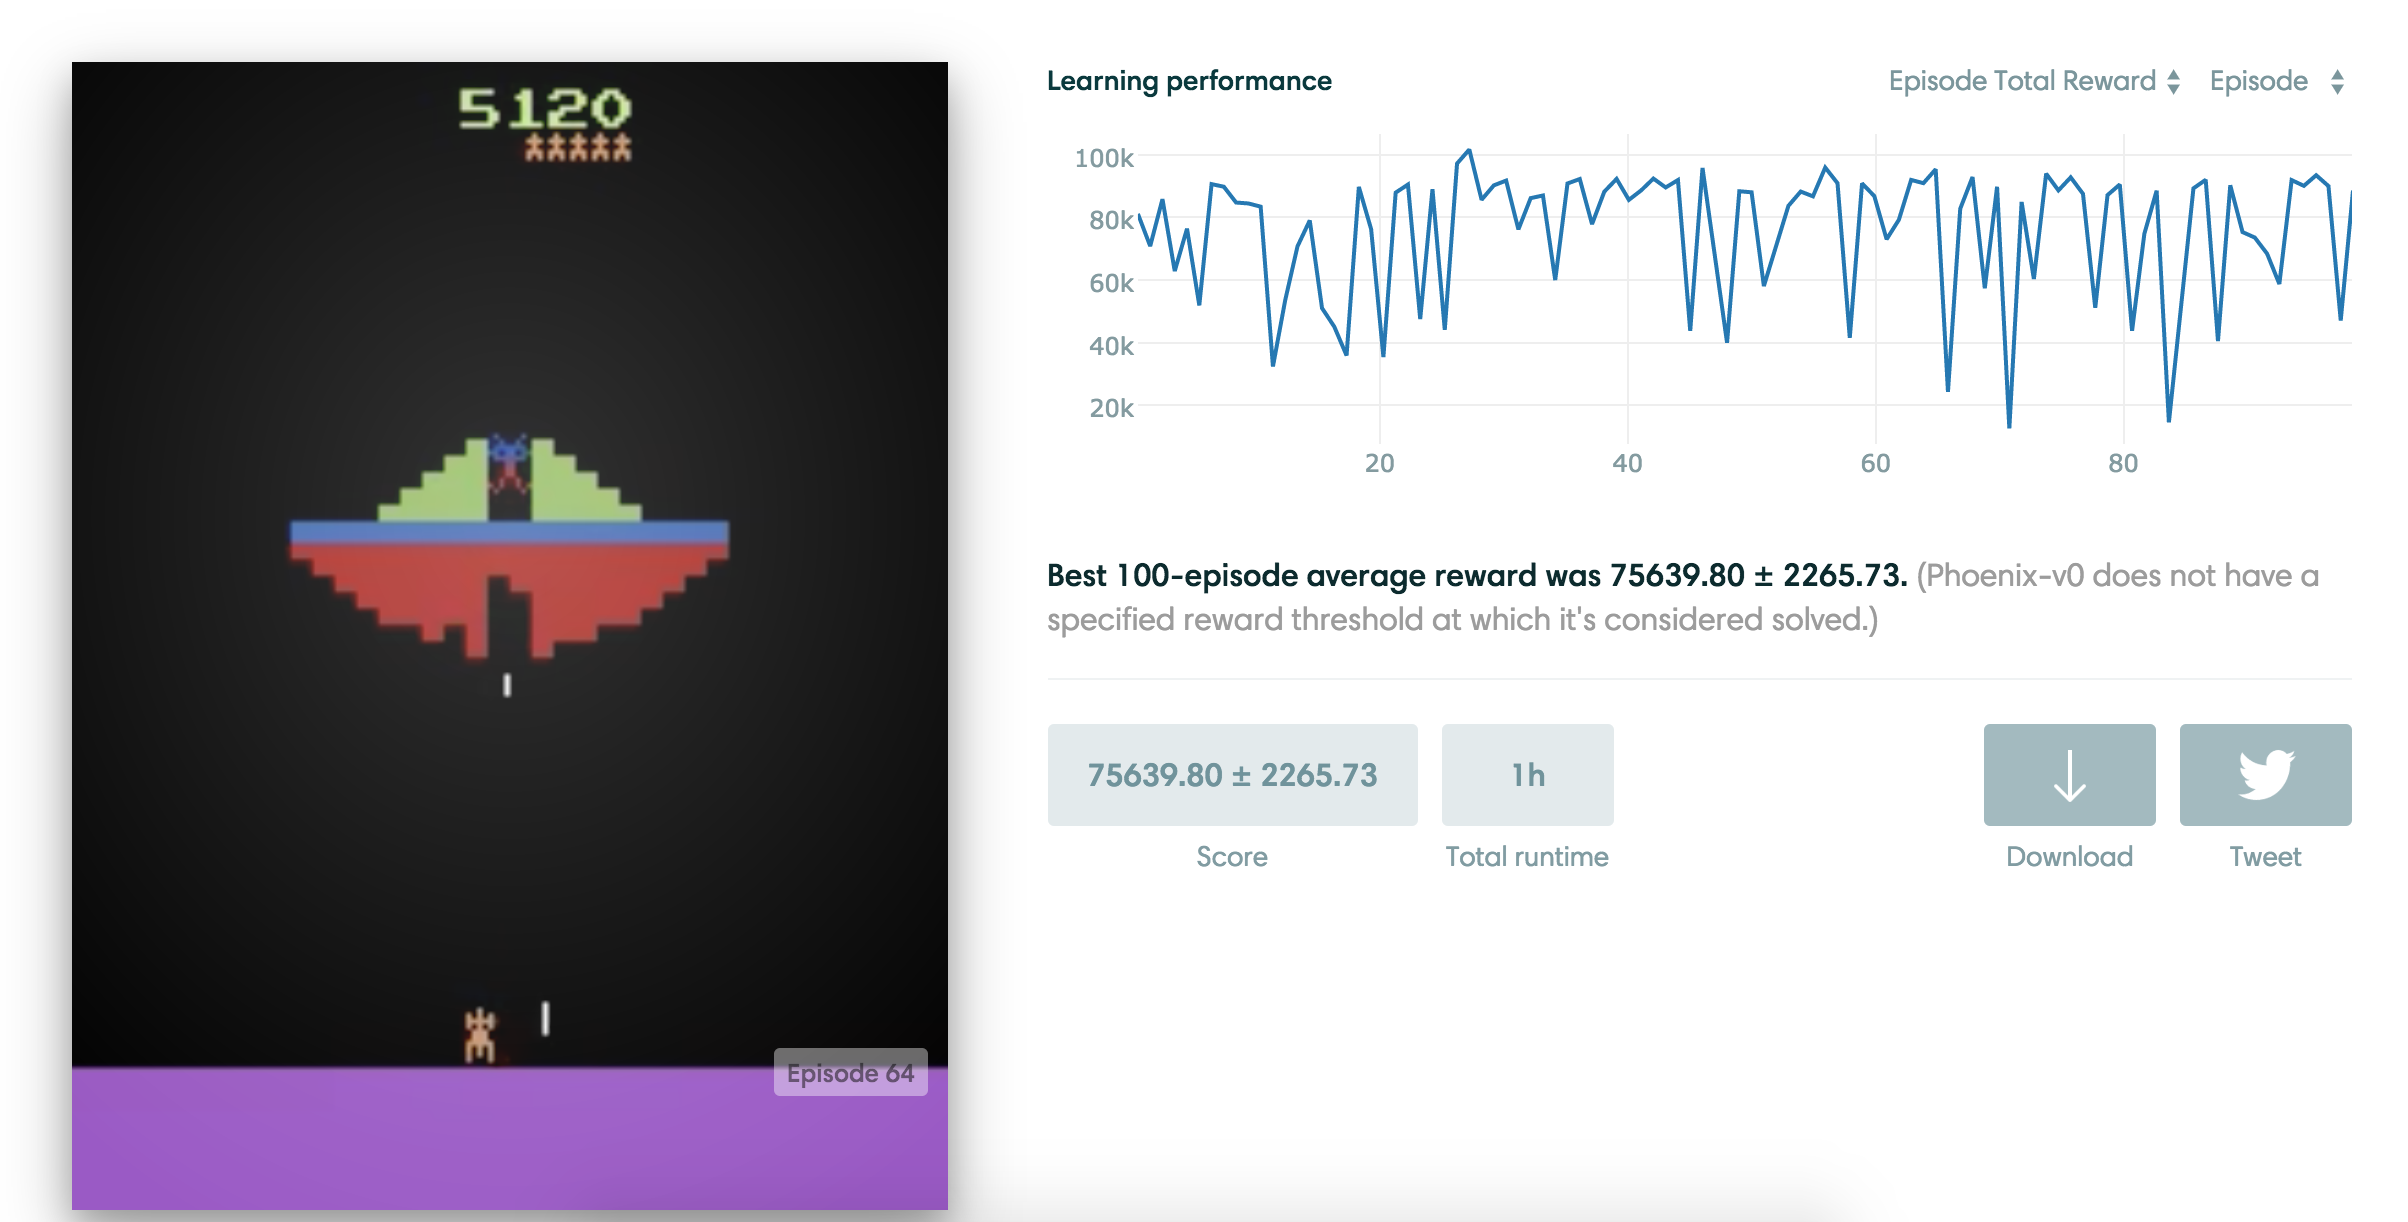
\includegraphics[width=0.49\textwidth]{./fig/A3C_Phoenix-v0.png} \\
% (c) \href{https://gym.openai.com/evaluations/eval_Gva8XrEvTQi63KOd5Gyq1Q#reproducibility}{Phoenix-v0} \\
% \end{tabular}
% \caption{The results of 100 epsiodes on three environments by applying A3C algorithms. By clicking the name of each environment 
% beneath the figures, you will see the video for each game played by trained agent.}
% \label{fig:A3C_baselines}
% \end{figure}



